%%%%%%%%%%%%%%%%%%%%%%%%%%%%%%%%%%%%%%%%%%%%%%%%%%%%%%%%%%%%%%%%%%%%%%%%%%%%%%%%
% TUM-Vorlage: Präsentation - Beispiele
%%%%%%%%%%%%%%%%%%%%%%%%%%%%%%%%%%%%%%%%%%%%%%%%%%%%%%%%%%%%%%%%%%%%%%%%%%%%%%%%


%%%%%%%%%%%%%%%%%%%%%%%%%%%%%%%%%%%%%%%%%%%%%%%%%%%%%
%% Folie: Gültigkeit der Masterfolien              %%
%%%%%%%%%%%%%%%%%%%%%%%%%%%%%%%%%%%%%%%%%%%%%%%%%%%%%

%%%%%%%%%%%%%%%%%%%%%%%%%%%%%%%%%%%%%%%%%%%%%%%%%%%%%
%% Folie: Grundlage der Masterfolien               %%
%%%%%%%%%%%%%%%%%%%%%%%%%%%%%%%%%%%%%%%%%%%%%%%%%%%%%

%%%%%%%%%%%%%%%%%%%%%%%%%%%%%%%%%%%%%%%%%%%%%%%%%%%%%
%% Folie: 2-zeilige Überschrift                    %%
%%%%%%%%%%%%%%%%%%%%%%%%%%%%%%%%%%%%%%%%%%%%%%%%%%%%%


\begin{frame}
\shiftedframetitle{Motivation}

\begin{itemize}
    \item Web latency and security are becoming more and more important.
    
    \item Middleboxes have caused a protocol ossification. Attempted extensions to TCP like TCP Fast Open\cite{DBLP:conf/conext/RadhakrishnanCCJR11}, SCTP\cite{rfc3286}, Multipath TCP \cite{rfc6824} have not seen widespread deployment.
    
    \item QUIC is a user-space transport protocol built on top of UDP. Also QUIC provides for authen
    ticated, encrypted header and payload which avoids dependency on vendors
    and ISPs
    
    \item Google started work on QUIC in 2012. 
    
    \item Faster development and deployment cycles. Already on Q044 version and accounts for more than 35\% of
    Google’s total egress traffic and 7\% of global internet traffic.
    
    \item  QUIC has been shown to reduce search latency by 8\% for desktop users and 3.6\% for mobile users.\cite{DBLP:conf/sigcomm/LangleyRWVKZYKS17}
    
    \item An IETF working group has been
    formed to standardize QUIC which should lead to even greater adoption.
    
\end{itemize}
\end{frame}
\clearpage


\begin{frame}
\shiftedframetitle{Goal and Approach}
\begin{itemize}
    
    \item Initial performance results from Google showed great gains but there is still a lack
    of repeatable studies.
    
    \item Rapid development cycle of QUIC means
    that many new features are introduced in each version of QUIC and support for older
    versions is dropped. So previous studies become obsoleted quickly.
    
    \item In this thesis we aim to evaluate the performance of QUIC(Q035, Q039, Q043, Q044) and compare it with
    TCP/TLS. 
    
    \item To do this we conduct experiments on real Internet to investigate connection
    establishment time, Time to first byte, download time, YouTube QoE metrics, Throughput,
    fairness in competing flow scenarios and CPU utilization.
    
\end{itemize}
\end{frame}
\clearpage

\begin{frame}
    \shiftedframetitle{Goal and Approach}
    \begin{itemize}
        \item\textbf{RQ1 : How do different versions of QUIC compare with each other and TCP/TLS 1.2 and TCP/TLS 1.3 on IPv4 and IPv6?}
% Newer versions of QUIC(Q044) should ideally provide some improvement over older ones(Q043, Q039, Q035).
        
        \item\textbf{RQ2 : How do the versions of QUIC compare with each other on different Autonomous Systems?}

        \item\textbf{RQ3 : How does throughput and CPU utilization of QUIC compare with TCP/TLS?}
        
        
        \item\textbf{RQ4 : Is QUIC fair towards TCP/TLS?}
        
    \end{itemize}
\end{frame}
\clearpage



\begin{frame}
\shiftedframetitle{Background}
SPDY is the first attempt by Google to improve Web Latency.\cite{spdy} HTTP/2 is the successor of SPDY protocol.

It has features like multiplexing requests over a single TCP connection, HTTP header compression, request prioritization, server push and server hint\cite{rfc7540}

HTTP/2 suffers from the TCP head-of-line blocking issue.

Previous work \cite{DBLP:conf/networking/El-khatibTW14}\cite{7745823}\cite{DBLP:conf/sac/CarlucciCM15}\cite{DBLP:conf/icc/MegyesiKM16} shows the improvements provided by SPDY and HTTP/2.  

    QUIC has many innovative features like Version Negotiation, 0-RTT connection establishment, Reduced head-of-line blocking, improved congestion control using packet pacing, Authenticated, encrypted header and payload, stream multiplexing, Connection-IDs, stream and connection level flow control, connection migration and resilience to NAT rebinding.\cite{ietf-quic-transport-18}

\end{frame}
\clearpage

\begin{frame}
    \shiftedframetitle{Background}
QUIC replaces most of the traditional HTTPS stack: TCP, TLS, HTTP/2.
\begin{figure}[!t]
    \centering
    \minipage{0.5\textwidth}
    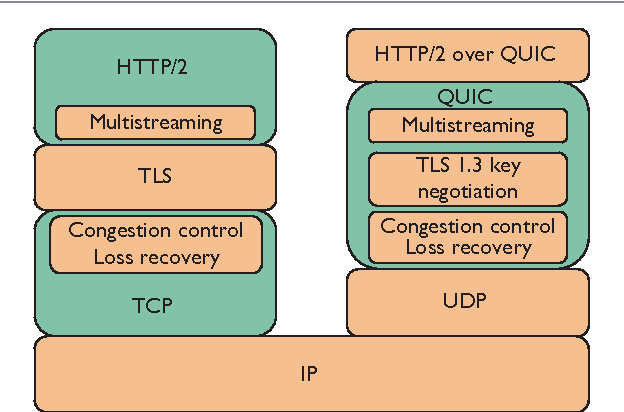
\includegraphics[width=1\textwidth]
    {figures/QUICstack.png}
    \endminipage\hfill
    \caption{\label{fig:QUIC_architecture}Layered QUIC architecture in the traditional HTTPS stack. QUIC incorporates features of congestion control, loss recovery similar to TCP, Multiple streams like HTTP2 and key negotiation like TLS.\cite{Cui2017}}
    
\end{figure}
\end{frame}
\clearpage

\begin{frame}
    \shiftedframetitle{Connection Establishment\cite{DBLP:conf/sigcomm/LangleyRWVKZYKS17}\cite{quicgd}\cite{crypto}}
    
    \begin{figure}[!ht]
        \centering
        \minipage{0.5\textwidth}
        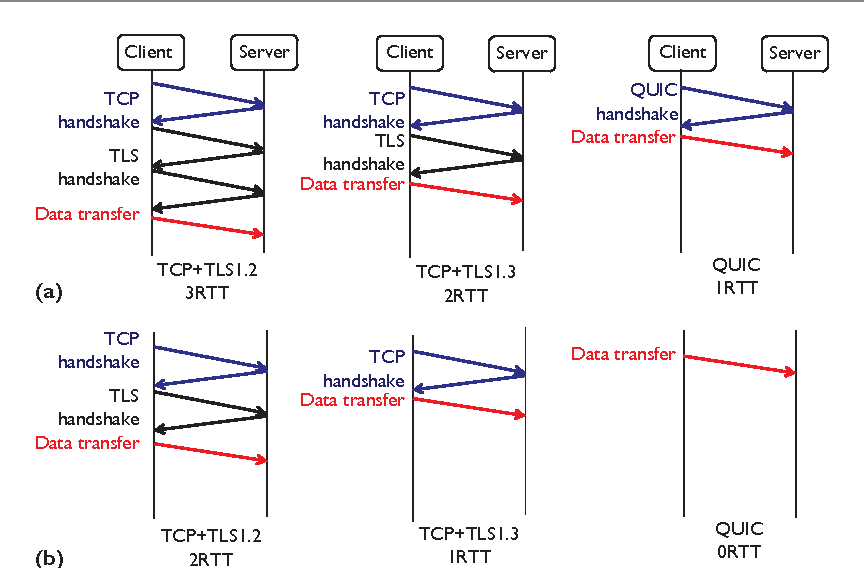
\includegraphics[width=1\textwidth]
        {figures/0rtt.png}
        \endminipage\hfill
        \caption{\label{fig:RTT} Handshake round-trip time (RTT) of different protocols. (a) First-time connection establishment. (b) Subsequent connections.\cite{Cui2017}}
    \end{figure}

    
    
\end{frame}
\clearpage

\begin{frame}
    \shiftedframetitle{Multiplexing}
    \begin{figure}[!ht]
        \centering
        \minipage{0.5\textwidth}
        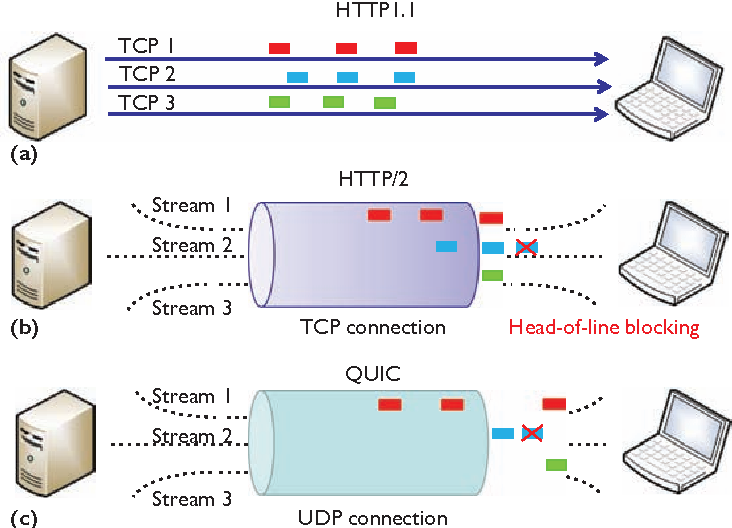
\includegraphics[width=1\textwidth]
        {figures/hol.png}
        \endminipage\hfill
        \caption{\label{fig:hol}Multiplexing comparison. This involved sending multiple streams of data over a single transport connection using (a) HTTP1.1, (b) HTTP/2, and (c) QUIC.\cite{Cui2017}}
    \end{figure}

QUIC also supports multiple streams in a single connection but the packets can be delivered out of order and a lost packet affects only those streams whose data it carried, not affecting other streams.


\end{frame}
\clearpage

\begin{frame}
    \shiftedframetitle{Congestion Control + Packet Pacing}
    
        \begin{figure}[!ht]
        \centering
        \minipage{0.7\textwidth}
        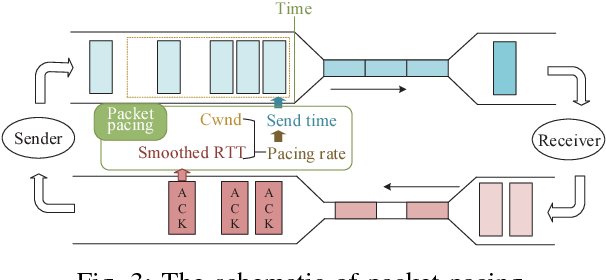
\includegraphics[width=1\textwidth]
        {figures/pacing.png}
        \endminipage\hfill
        \caption{\label{fig:pacing}Packet Pacing \cite{DBLP:conf/ipccc/YuXY17}}
    \end{figure}

Default congestion control algorithm is CUBIC\cite{DBLP:journals/internet/CuiLLWK17} but differs from TCP CUBIC slightly.\cite{quicgd}\cite{ietf-quic-recovery-18}. BBR is a new congestion control algorithm being developed by Google.\cite{DBLP:conf/pam/LiCJC18}

Packet Pacing is done by inserting a waiting time between each UDP datagram (enabled by default)
This helps lower retransmission rate \cite{DBLP:conf/infocom/AggarwalSA00}

\end{frame}
\clearpage

\begin{frame}
\shiftedframetitle{Prior Work}
    Langley et al. \cite{DBLP:conf/sigcomm/LangleyRWVKZYKS17} discuss about motivations in various design decisions of QUIC, development and testing performed over various iterations, performance improvements. They provide us with the first large-scale measurements of QUIC across various versions.
    
    Nepomuceno et al.\cite{8538687}, Cook et al.\cite{DBLP:conf/icc/CookMTH17} look at page load time.
    
    Li et al.\cite{DBLP:conf/pam/LiCJC18}, Kharat et al.\cite{8524247}, Qian et al. \cite{DBLP:journals/access/QianWT18}, Kakhki et al.\cite{DBLP:conf/imc/KakhkiJCNM17}look at throughput, congestion control and fairness among flows.
    
    Yu et al. \cite{DBLP:conf/ipccc/YuXY17} focused mainly on packet pacing mechanism for congestion control.
    
    Saverimoutou et al.\cite{DBLP:conf/iscc/SaverimoutouMV17}, Fischlin et al.\cite{DBLP:conf/ccs/FischlinG14} and Vaere et al.\cite{DBLP:conf/imc/VaereBKT18} look into the security aspects of QUIC.
    
    Willem et al.\cite{udpgso} and Edeline et al. \cite{DBLP:journals/corr/EdelineKTAD16} look into how QUIC being built on top of UDP affects it.
    
    Wang et al.\cite{DBLP:conf/mswim/WangBRP18} implement QUIC in the linux kernel and perform experiments to compare both in kernel mode.

    Rüth et al.\cite{DBLP:conf/pam/RuthPDH18} look into QUIC usage in the wild.

     
\end{frame}
\clearpage

\begin{frame}
\shiftedframetitle{Methodology}

\end{frame}
\clearpage

\begin{frame}
\shiftedframetitle{Overview of Thesis Results}

\end{frame}
\clearpage

\begin{frame}
\shiftedframetitle{Conclusion}

\end{frame}
\clearpage


\begin{frame}
\shiftedframetitle{Future work and limitations}
\begin{itemize}
    
    \item Geographical bias due to location of probes.For more representative results the tests should be deployed at multiple locations with the help of CAIDA Ark \cite{CAIDAArk} measurement infrastructure and SamKnows project\cite{SamKnowsproject}
    
    \item Mobile devices are a major source of QUIC traffic so tests need to be adopted for mobile devices using cronet\cite{cronet}.
    
    \item No support for 0-RTT connections in lsquic at the time of test creation. Support has been introduced in latest release.
    
    \item The QUIC \texttt{YouTube tests} have a higher failure rate than TCP \texttt{YouTube tests} which can be looked into.
    
    \item Other features of QUIC like Congestion control window size, Packet pacing, Flow control can be evaluated.
    
    \item  QUIC tests can be performed under constrained conditions like low buffer size, introducing random bandwidth changes, random packet loss and different RTTs.
    
    \item  Other metrics like no. of retransmissions, no. of packets lost, congestion window size can be measured.
    
    \item IETF QUIC may be standardized soon, it may also be considered for comparison with Google QUIC and TCP/TLS.
    

\end{itemize}
\end{frame}
\clearpage
